\begin{frame}
	\frametitle{Wikipedia}

	\begin{itemize}
		\item Online Lexikon
		\item Gründung 15. Januar 2001
		\item Platz 6 (deu:8) meistbesichte Websites
		\item > 39,5 Mio Artikel in ca. 300 Sprachen
	\end{itemize}

	Quelle: \href{https://de.wikipedia.org/wiki/Wikipedia}{Wikipedia} (Juni 2016)
\end{frame}

\begin{frame}
	\frametitle{riseup.net}
	
	\begin{itemize}
		\item Mail-Account u. -Listen Provider
		\item Secure Internet Live Conferencing
		\item VPN, Wiki, Pad, Speicher, …
	\end{itemize}
	
	Quelle: \href{https://riseup.net/}{riseup.net}
\end{frame}

\begin{frame}
	\frametitle{Experimental living}
	
	\begin{figure}
		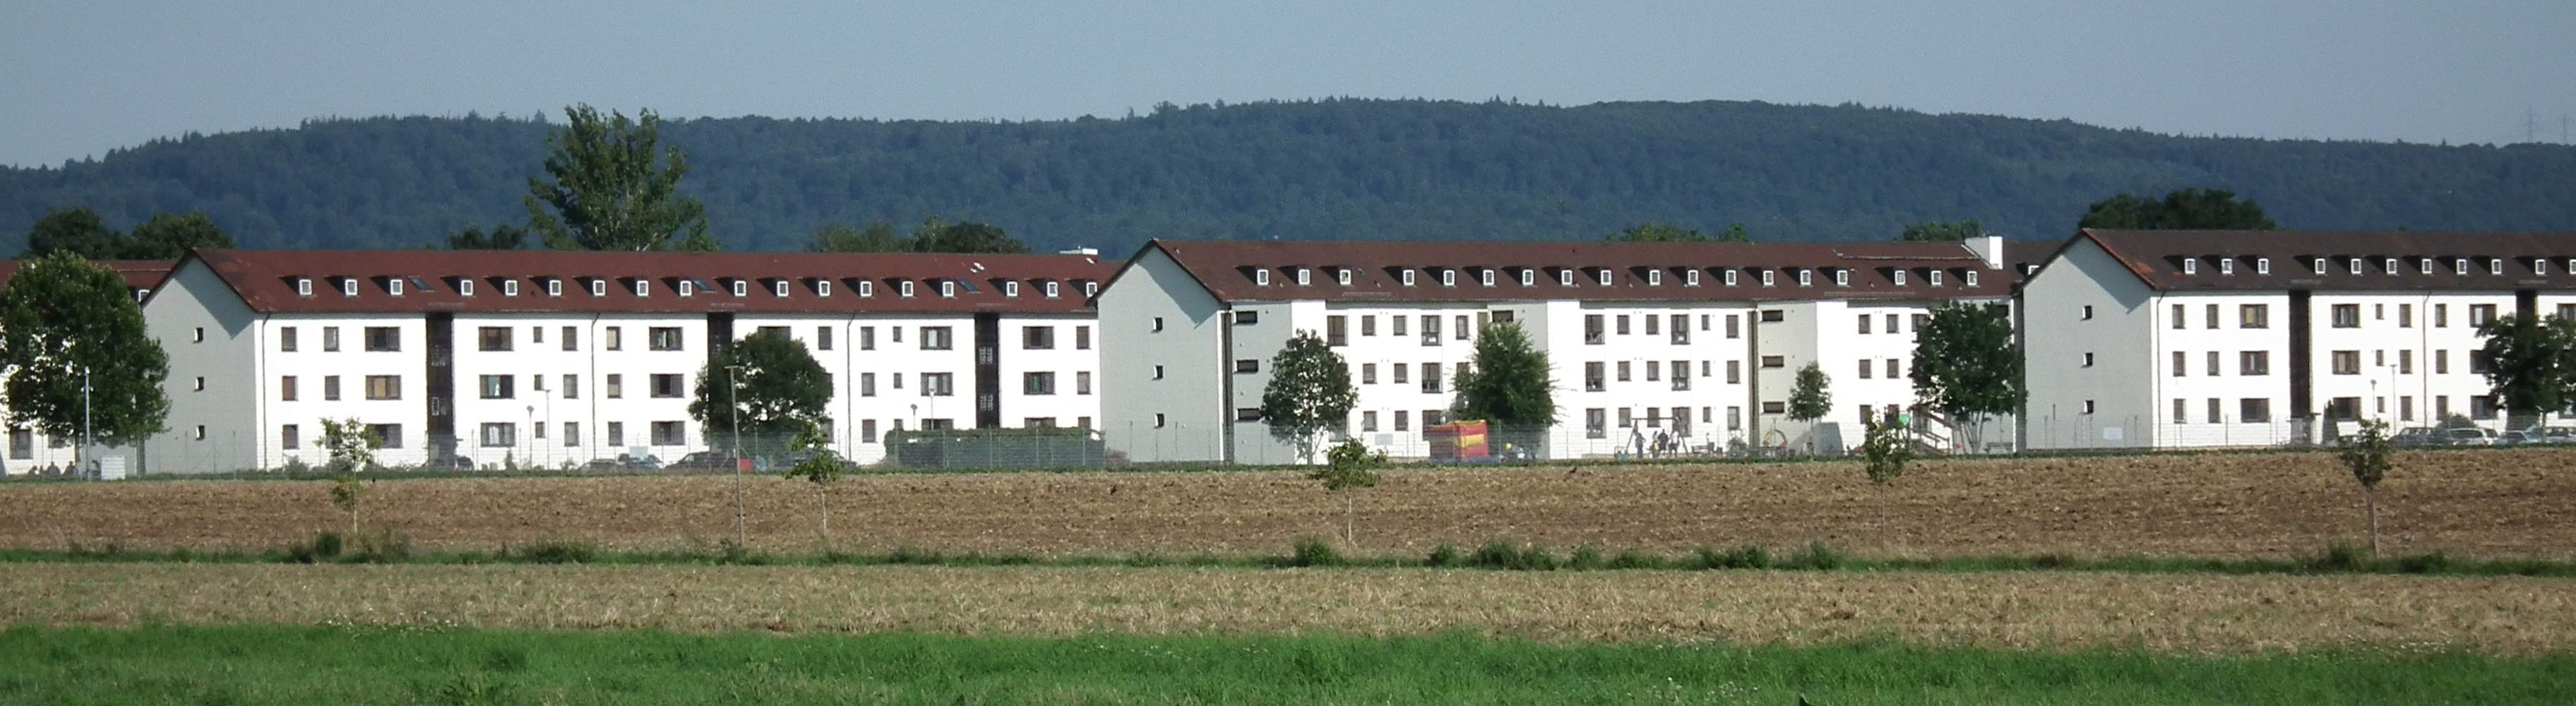
\includegraphics[height=0.2\textheight]{img/Wohnhaeuser_PHV_cut.jpg}
		\caption[Blick von Norden auf PHV, Ausschnitt]{\href{https://de.wikipedia.org/wiki/Datei:Wohnh\%C3\%A4user_PHV.JPG}{User:4028mdk09, CC BY-SA 3.0}}
	\end{figure}
	
	\begin{itemize}
		\item Carlo Ratti für IBA Heidelberg
		\item Smart City
		\item co-living, co-working, co-making
	\end{itemize}

	Quelle: \href{https://de.wikipedia.org/wiki/Patrick-Henry-Village}{Wikipedia:PHV}, \hspace{1cm}
	\href{http://www.carloratti.com/project/patrick-henry-commune/}{Carlo Ratti}, \\
	\href{http://www.bbc.co.uk/news/technology-37510322}{The village that just wants to share}
\end{frame}

